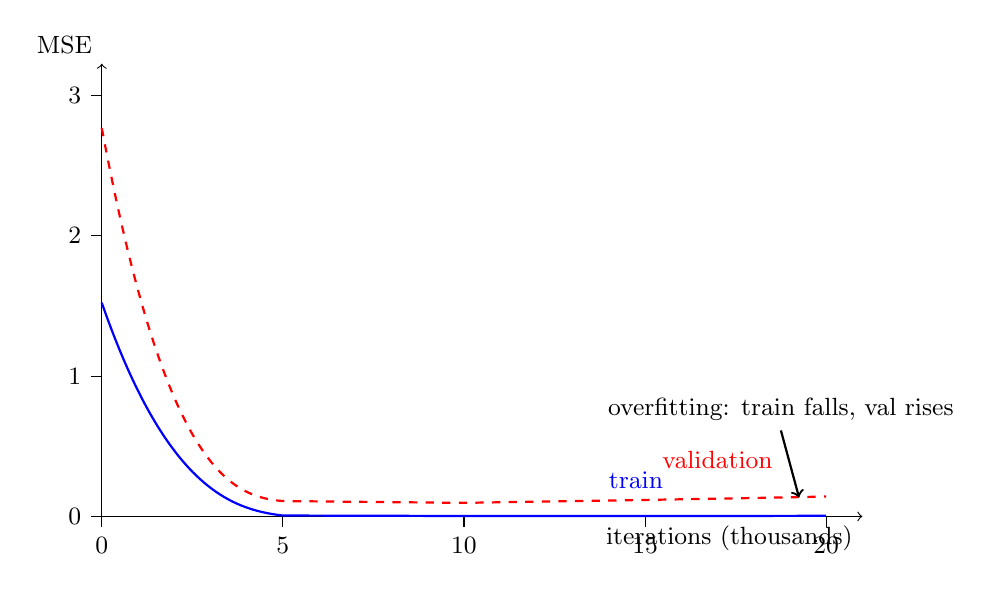
\begin{tikzpicture}[scale=1.15]
% train/val loss curves of TinyNet — REAL numbers from ch14_tinynet.py
% y scale: MSE v -> 1.55*v ; x scale: 1000 iters -> 0.4
\draw[->] (0,0)--(8.4,0) node[below left]{\small iterations (thousands)};
\draw[->] (0,0)--(0,5.0) node[above left]{\small MSE};
\foreach \v/\y in {0/0,1/1.55,2/3.10,3/4.65} {
  \draw (0,\y) -- (-0.12,\y) node[left]{\small \v}; }
\foreach \t/\x in {0/0,5/2.0,10/4.0,15/6.0,20/8.0} {
  \draw (\x,0) -- (\x,-0.12) node[below]{\small \t}; }
% train: (0,1.5247)(5000,.0038)(10000,.0029)(15000,.0026)(20000,.0042)
\draw[thick,blue] (0,2.36) .. controls (0.7,0.35) and (1.4,0.08) .. (2.0,0.01)
  .. controls (3.0,0.005) .. (4.0,0.005) -- (6.0,0.004) -- (8.0,0.007);
\node[blue] at (5.9,0.40) {\small train};
% val: (0,2.7691)(5000,.1074)(10000,.098)(15000,.1295)(20000,.1412)
\draw[thick,red,dashed] (0,4.29) .. controls (0.7,0.55) and (1.4,0.22) .. (2.0,0.17)
  .. controls (3.0,0.15) .. (4.0,0.15)
  .. controls (5.2,0.17) and (6.6,0.19) .. (8.0,0.22);
\node[red] at (6.8,0.62) {\small validation};
\draw[<-,thick] (7.7,0.21) -- (7.5,0.95) node[above]{\small overfitting: train falls, val rises};
\end{tikzpicture}
